\documentclass[main.tex]{subfiles}
% 向量函数及其图像
\begin{document}
在线性代数部分的介绍中,我们知道实数域$\mathbb{R}$上的$n$维向量空间的向量在给定基下总是唯一对应于$n$维实坐标空间$\mathbb{R}^n$中的一组有序实数$n$元组。因此,如不另作说明,向量函数都直接讨论$\mathbb{R}^n$上的向量。

\begin{definition}[向量函数]\label{def:II.4.1}
    从$\mathbb{R}^n$到$\mathbb{R}^m$的映射$\mathbf{f}:\mathbb{R}^n\supset D\rightarrow\mathbb{R}^m$是一个\emph{向量函数(vector function)}。其变量是一个$n$维向量空间的向量$\mathbf{r}\in\mathbb{R}^n$,$\mathbf{r}=\left(r_1,\cdots,r_n\right)^\intercal$;其像(函数值)$\mathbf{f}\left(\mathbf{r}\right)$是一个$m$维向量空间的向量$\mathbf{f}\left(\mathbf{r}\right)\in\mathbb{R}^m$,$\mathbf{f}\left(\mathbf{r}\right)=\left(f_1\left(\mathbf{r}\right),\cdots,f_m\left(\mathbf{r}\right)\right)^\intercal$。$f_j:\mathbb{R}_n\rightarrow\mathbb{R},j=1,\cdots,m$称为$\mathbf{f}$的\emph{坐标函数(coordinate function)}。
\end{definition}



\begin{example}\label{exp:II.4.1}
    函数$\mathbf{f}:\mathbb{R}^3\rightarrow\mathbb{R}^2$,
    \[\begin{split}\mathbf{f}\left(\mathbf{r}\right)=\left(\begin{array}{c}r_1^2+r_2^2+r_3^2\\r_1+r_2+r_3\end{array}\right)=\left(\begin{array}{c}f_1\\f_2\end{array}\right),\\f_1\leq0,f_2\in\mathbb{R}\end{split}\]
    其中$\mathbf{r}=\left(r_1,r_2,r_3\right)^\intercal\in\mathbb{R}^3$,$\mathbf{f}=\left(f_1,f_2\right)^\intercal\in\mathbb{R}^2$。以往我们更习惯把上述函数写成:
    \[
        \left\{\begin{array}{l}
            P\left(x,y,z\right)=x^2+y^2+z^2 \\
            Q\left(x,y,z\right)=x+y+z
        \end{array}
        \right.
    \]
\end{example}

\begin{example}\label{exp:II.4.2}
    函数$\mathbf{A}:\mathbb{R}^3\rightarrow\mathbb{R}^2$,
    \[\mathbf{A}\left(\mathbf{r}\right)=\left(\begin{array}{c}3r_1+4r_2\\3r_2+5r_3\end{array}\right)=\left(\begin{array}{ccc}3&4&0\\0&3&5\end{array}\right)\left(\begin{array}{c}r_1\\r_2\\r_3\end{array}\right)\]
    是一个线性变换,又称线性函数。线性函数也可以按线性代数的惯例记为:$\mathbf{Ar}$。
\end{example}

\begin{definition}[隐函数]\label{def:II.4.2}
    考虑函数$\mathbf{F}:\mathbb{R}^{n+m}\rightarrow\mathbb{R}^m$,若将$\mathbb{R}^{n+m}$中的元素$\left(x_1,\cdots,x_n,y_1,\cdots,y_m\right)^\intercal$写成$\left(\mathbf{x},\mathbf{y}\right)^\intercal$,其中$\mathbf{x}=\left(x_1,\cdots,x_n\right)^\intercal$,$\mathbf{y}=\left(y_1,\cdots,y_m\right)^\intercal$,则$\mathbf{F}\left(\mathbf{r}\right),\mathbf{r}\in\mathbb{R}^{n+m}$也可写成$\mathbf{F}\left(\mathbf{x},\mathbf{y}\right)$。若函数$\mathbf{f}:\mathbb{R}^n\supset D\rightarrow\mathbb{R}^m$满足方程$\mathbf{F}\left(\mathbf{x},\mathbf{f}\left(\mathbf{x}\right)\right)=\mathbf{0},\forall\mathbf{x}\in D$则称这一方程\emph{隐含地定义了(implicitly defined)}函数$\mathbf{f}$。用这种方式表示的函数叫\emph{隐函数(implicit function)}。
\end{definition}

\begin{example}\label{exp:II.4.3}
    设函数$F\left(x,y\right)=x^2+y^2-1=0$,则“$F\left(x,f\left(x\right)\right)=x^2+\left(f\left(x\right)\right)^2-1=0,\forall x\in\mathrm{dom}f$”隐含地定义了以下任一函数:
    \begin{align*}
        f_1\left(x\right) & =\sqrt{1-x^2},\quad -1\leq x\leq 1                \\
        f_2\left(x\right) & =-\sqrt{1-x^2},\quad -1\leq x\leq 1               \\
        f_3\left(x\right) & =\left\{\begin{array}{ll}
                                        \sqrt{1-x^2},  & -\frac{1}{2}\leq x\leq 0 \\
                                        -\sqrt{1-x^2}, & 0\leq x\leq 1
                                    \end{array}\right.
    \end{align*}
\end{example}
由例\ref{exp:II.4.3}可见,不同定义域的函数$\mathbf{f}$都可由同一函数$\mathbf{F}$隐含地定义。函数的隐含定义并不完全确定该函数。

\begin{definition}[函数的图像]\label{def:II.4.3}
    函数$\mathbf{f}:\mathbb{R}^n\rightarrow\mathbb{R}^m$的\emph{图像(graph)}是指所有有序对$\left(\mathbf{r},\mathbf{f}\left(\mathbf{r}\right)\right)$的集合\cite[\S 6.4$\sim$6.7]{华工高数2009上}。
\end{definition}

图像的数学概念是一个集合,我们把图像画在纸上的方式只是一种惯例。具体地,函数$\mathbf{f}:\mathbb{R}^n\rightarrow\mathbb{R}^m$的图像是由所有满足
\[
    \left\{\begin{array}{c}y_1=f_1\left(x_1,\cdots,x_n\right)\\\vdots\\y_m=f_m\left(x_1,\cdots,x_n\right)\end{array}\right.
\]
的点$\left(x_1,\cdots,x_n,y_1,\cdots,y_m\right)$的集合(是$\mathbb{R}^{n+m}$的子集)。其中$f_1,\cdots,f_m$是$\mathbf{f}$的坐标函数。

我们只懂在纸上画出维数小于等于3的图形,即图上的任一点的坐标最多为3个实数。因此我们懂得在纸上画出的函数图像仅限$n+m\leq3$的情况。
\begin{example}\label{exp:II.4.4}
    函数$y=x^2-2$的图象是所有有序对$\left(x,y\right)$。同时,由于$\left(x,y\right)\in\mathbb{R}^2$,故这是平面上的图形。具体地,它是如图\ref{fig:II.4.1}所示的一条二次曲线。
\end{example}
\begin{figure}[h]
    \centering
    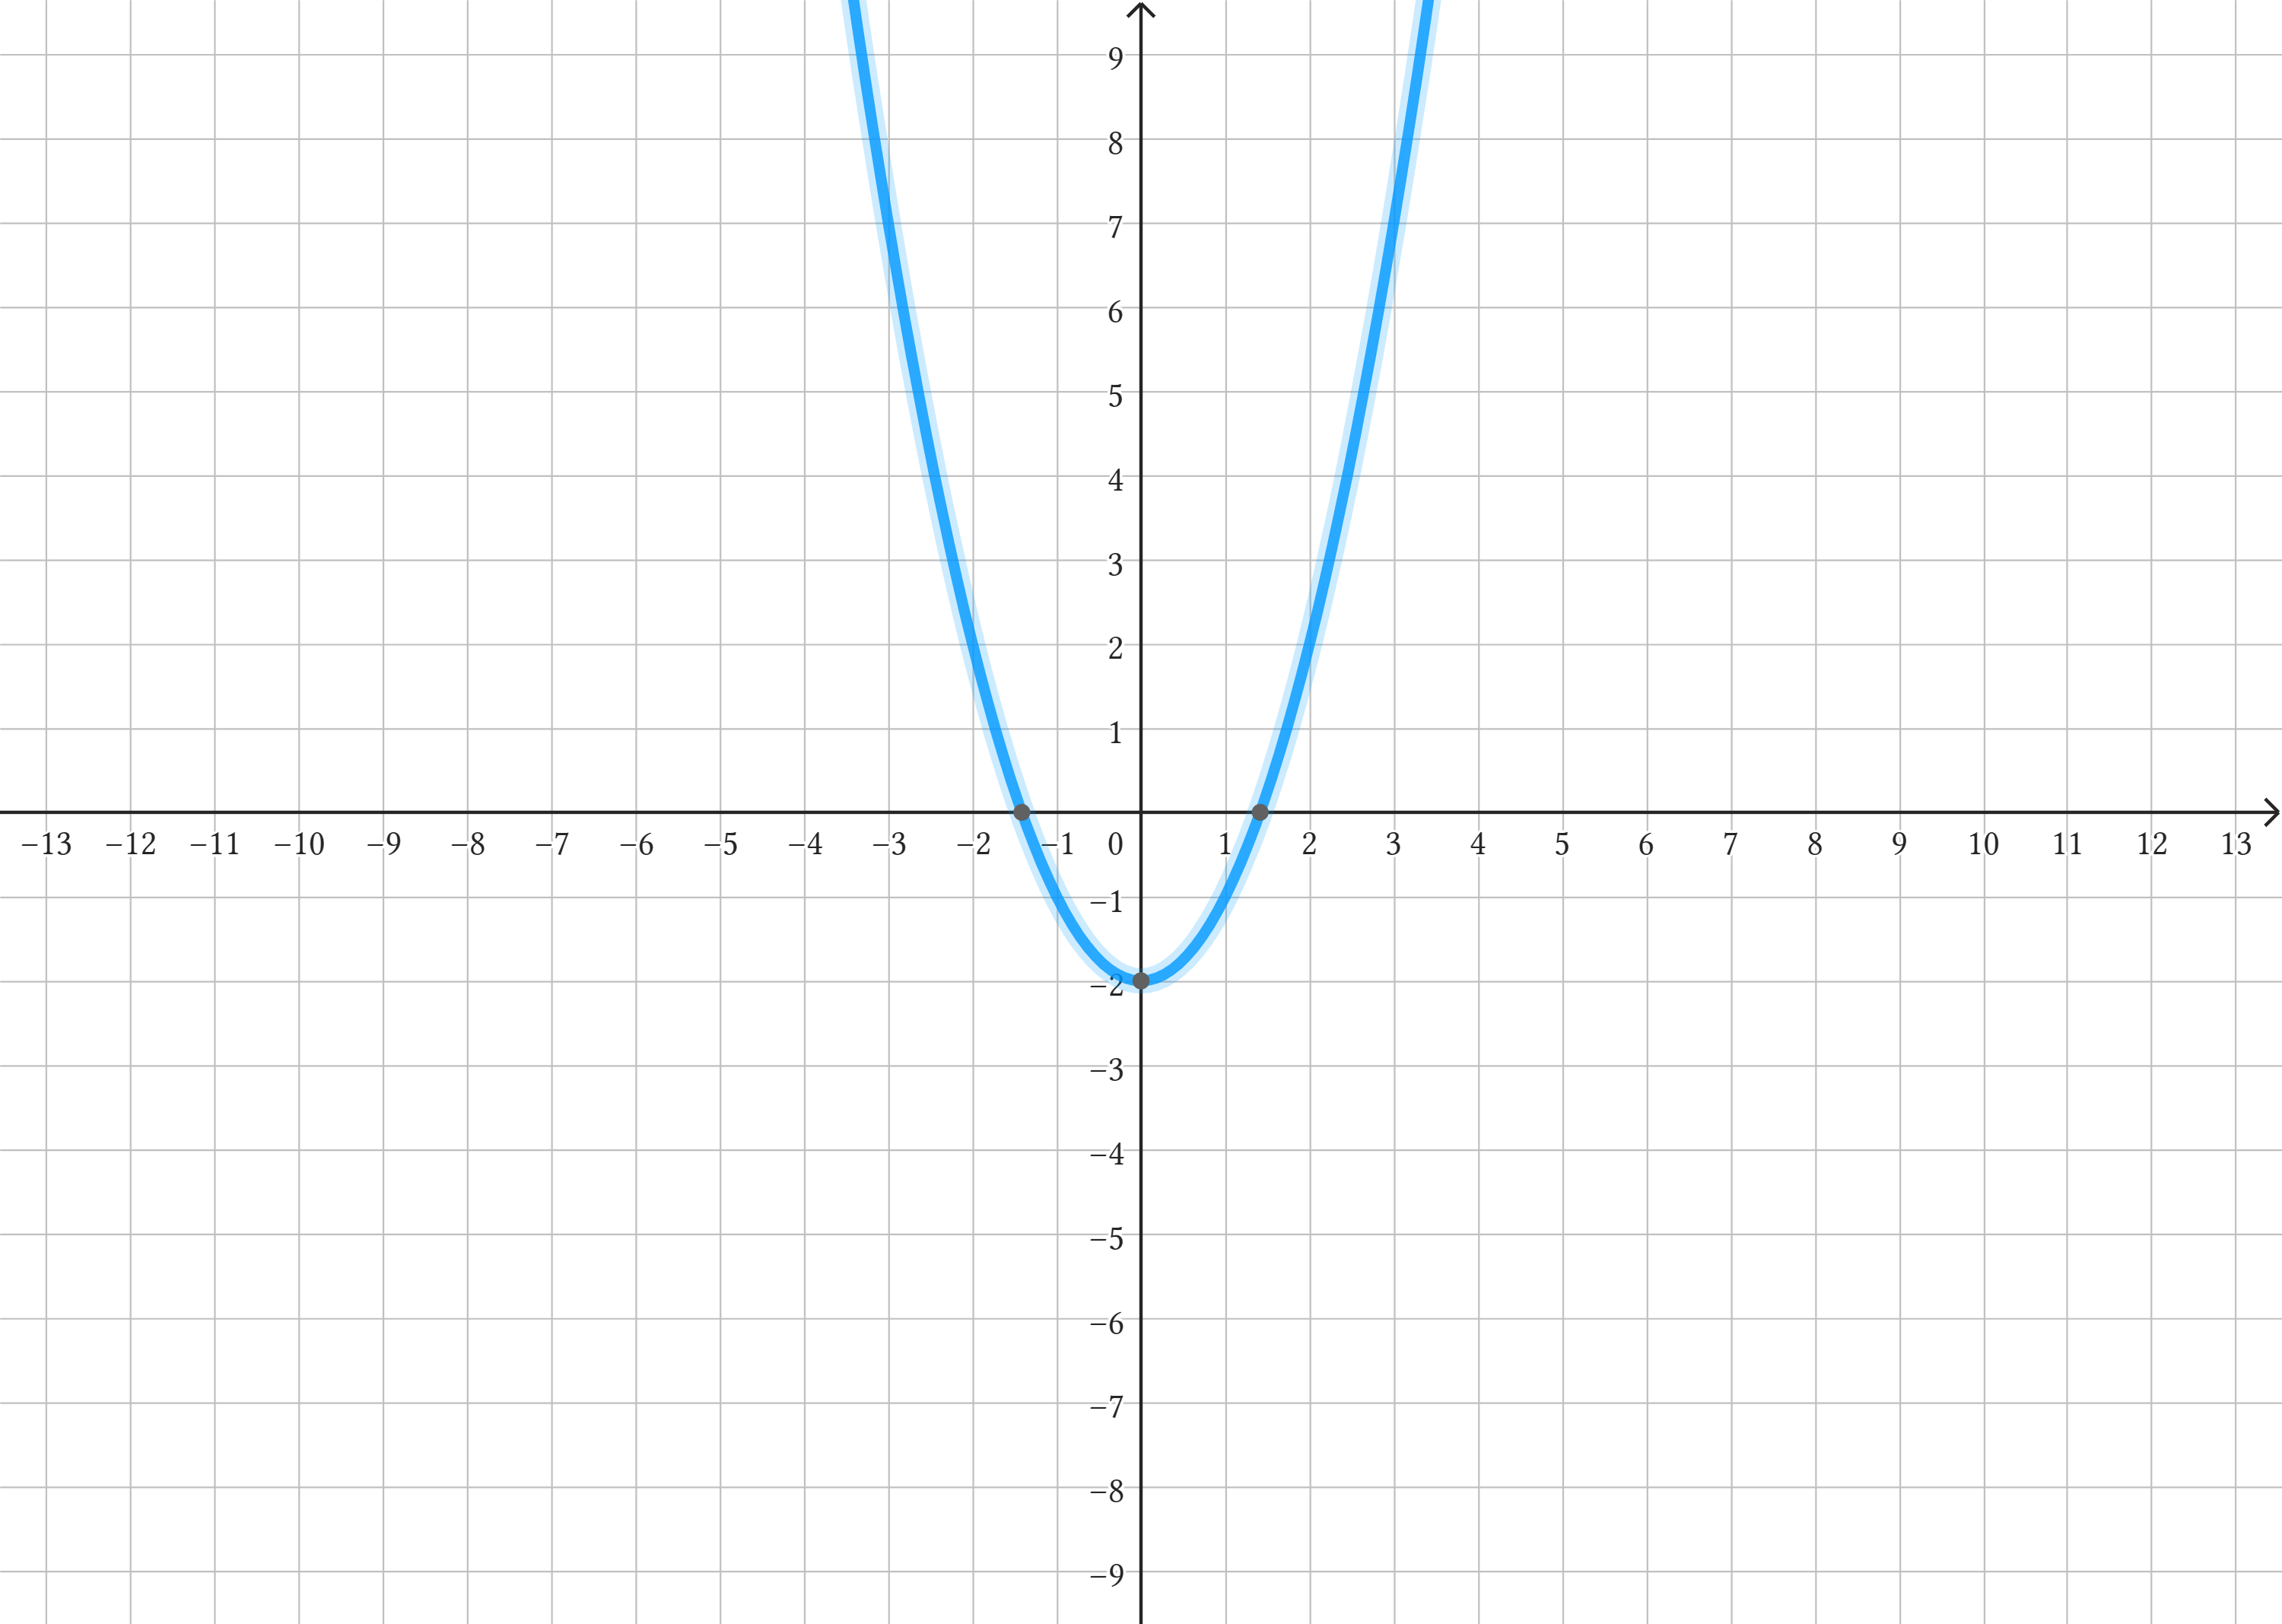
\includegraphics[width=0.5\textwidth]{images/II.4.1.png}
    \caption{函数$y=x^2-2$的图像。}
    \label{fig:II.4.1}
\end{figure}
\begin{example}\label{exp:II.4.5}
    函数$f:\mathbb{R}^2\rightarrow\mathbb{R},f\left(\mathbf{r}\right)=\left\|\mathbf{r}\right\|^2$的图像是有序3元组$\left(r_1,r_2,\left\|\mathbf{r}\right\|^2\right)$的集合,是3维空间的一个如图\ref{fig:II.4.2}所示的曲面。
\end{example}
\begin{figure}[h]
    \centering
    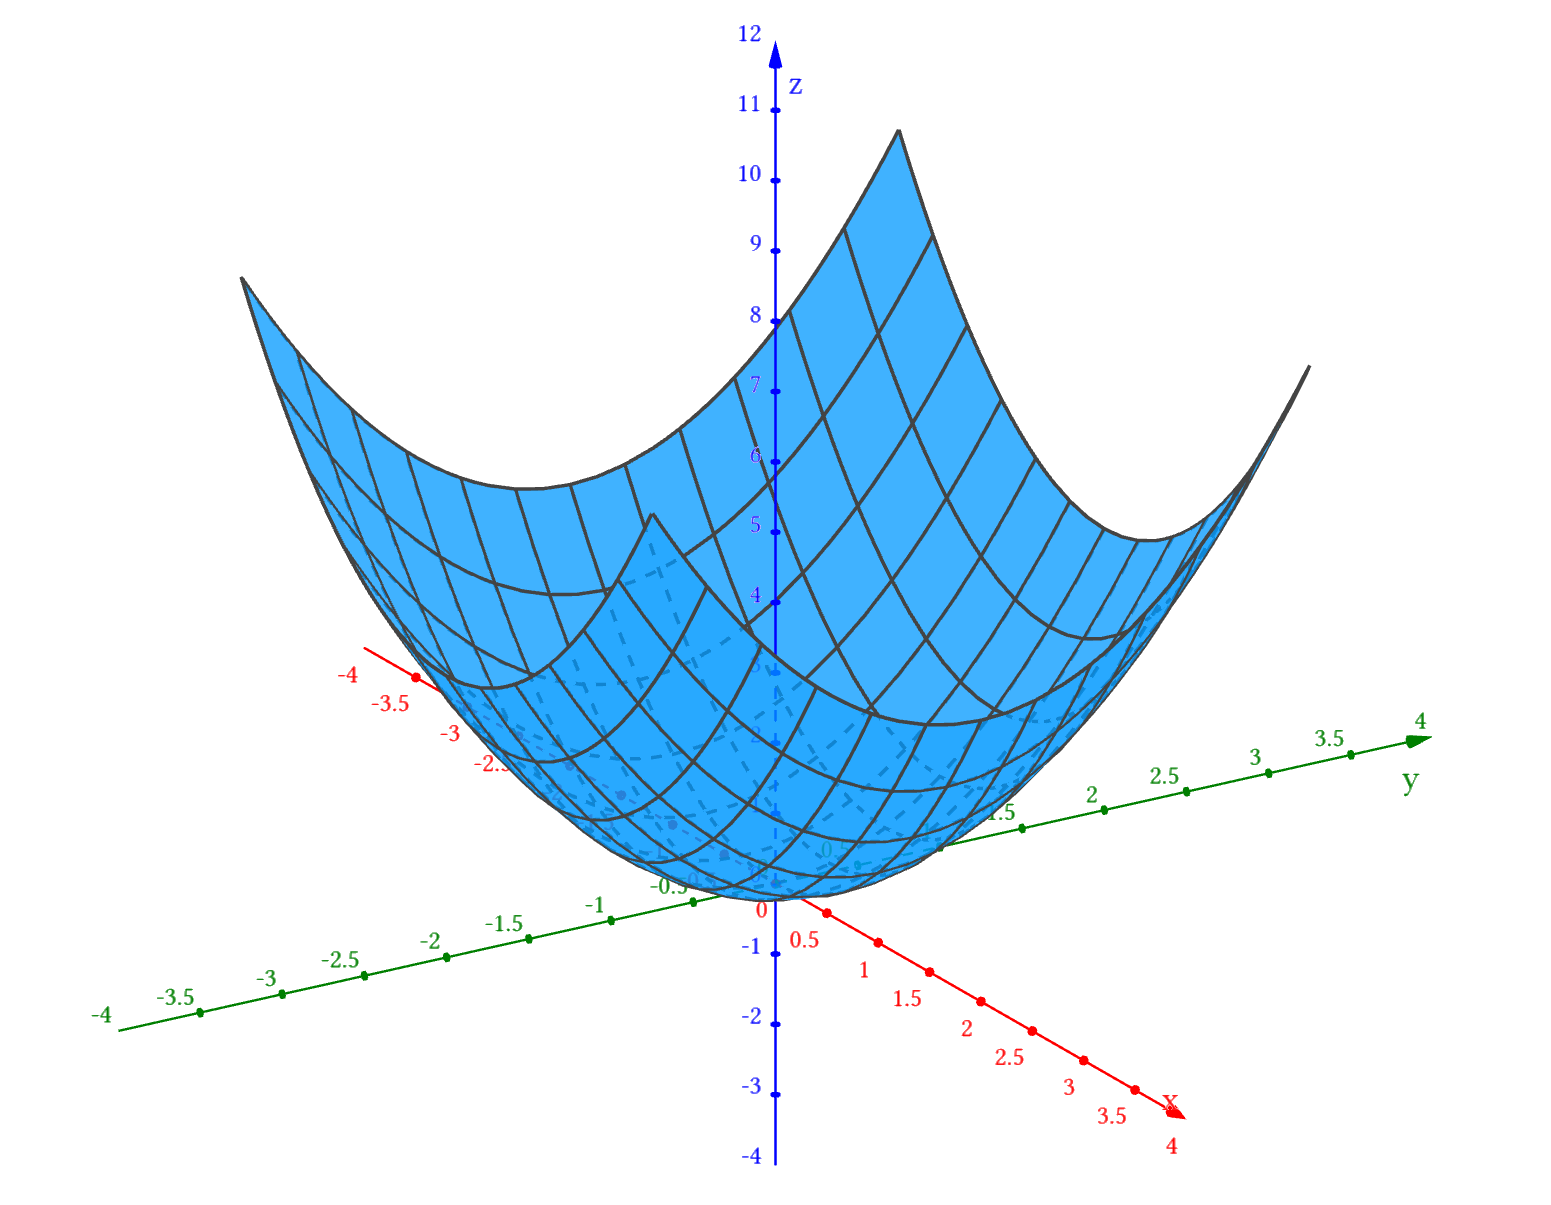
\includegraphics[width=0.5\textwidth]{images/II.4.2.png}
    \caption{函数$f:\mathbb{R}^2\rightarrow\mathbb{R},f\left(\mathbf{r}\right)=\left\|\mathbf{r}\right\|^2$的图像在$-2<r_1<2,-2<r_2<2$范围内的部分。}
    \label{fig:II.4.2}
\end{figure}
\begin{example}\label{exp:II.4.6}
    函数$\mathbf{f}:\mathbb{R}\rightarrow\mathbb{R}^2$,
    \[
        \mathbf{f}\left(t\right)=\left(\begin{array}{c}\cos t\\\sin t\end{array}\right),\quad\forall t\in\mathbb{R}
    \]
    的图像是所有有序对$\left(t,\left(\cos t,\sin t\right)\right)$。我们把2维向量$\left(\cos t,\sin t\right)$作在实数轴上$t$对应的位置,得到图\ref{fig:II.4.3}所示的螺线。
\end{example}
\begin{figure}[h]
    \centering
    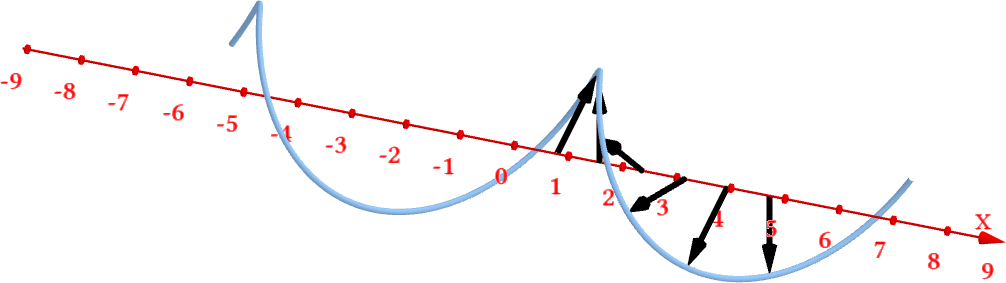
\includegraphics[width=0.75\textwidth]{images/II.4.3.png}
    \caption{例\ref{exp:II.4.6}函数的图象。}
    \label{fig:II.4.3}
\end{figure}
\begin{example}\label{exp:II.4.7}
    函数$f:\mathbb{R}^2\supset D\rightarrow\mathbb{R}^3,$
    \[
        \mathbf{f}\left(\mathbf{r}\right)=\left(\begin{array}{c}f_1\\f_2\\f_3\end{array}\right)=\left(\begin{array}{c}r_1\cos r_2\\r_1\sin r_2\\r_2\end{array}\right),\quad D: 0\leq r_1\leq 4,\leq r_2\leq 2\pi
    \]
    该函数的图像无法作成3维欧几里得空间中的点集,但我们仍可在3维欧几里得空间中对该函数进行可视化。我们看到,$\mathbf{f}$的定义域是2维平面上的一个矩形区域$D$。令$r_1=a$有
    \[
        \mathbf{f}=\left(\begin{array}{c}
                a\cos r_2 \\
                a\sin r_2 \\
                r_2
            \end{array}\right),\quad 0\leq r_2\leq 2\pi
    \]
    且$f_1^2+f_2^2=a^2$。视$a$为常数,则有序3元组$\left(a\cos r_2,a\sin r_2,r_2\right)$是一个螺线,其在$f_1-f_2$面上的投影是以原点为圆心、半径为$a$的圆。若令$r_2=\theta$,且$\theta$是常数,则有
    \[
        \mathbf{f}=\left(\begin{array}{c}
                r_1\cos \theta \\
                r_1\sin \theta \\
                \theta
            \end{array}\right),\quad 0\leq r_2\leq 2\pi
    \]
    且$f_1^2+f_2^2=r_1^2$。在同样的空间坐标上,这是螺线上某点到$z$轴的线段。随着$a$在$\left[0,4\right]$上变化、$\theta$在$\left[0,2\pi\right]$上变化,以原函数$\mathbf{f}\left(\mathbf{r}\right)$的坐标函数为坐标的点集是如图\ref{fig:II.4.4}所示的螺带曲面。但按定义\ref{def:II.4.3},这个曲面不是函数$\mathbf{f}$的图像。
\end{example}

例\ref{exp:II.4.7}中的函数按照图\ref{fig:II.4.4}可视化时,我们称这个三维空间中的螺带曲面是由一个\emph{参数方程(parametric equation)}(即$\mathbf{f}=\mathbf{f}\left(\mathbf{r}\right)$)所定义的曲面,它的\emph{参数变量(parametric variable)}$\mathbf{r}\in\mathbb{R}^2$取值的区域就是如图\ref{fig:II.4.4}所示的矩形区域,称为\emph{参数域(domain of parameter variable)}。我们所画出来的3维曲面只是函数$\mathbf{f}$的值域$\mathrm{ran}\mathbf{f}$所形成的点集。一般地,由参数方程$\mathbf{f}:\mathbb{R}^n\rightarrow\mathbb{R}^m$定义的几何形状,当$n=1$时,是$m$维空间中的曲线,$m=2,3$;当$n=2$时是$m=3$维空间中的曲面。

\begin{figure}[h]
    \centering
    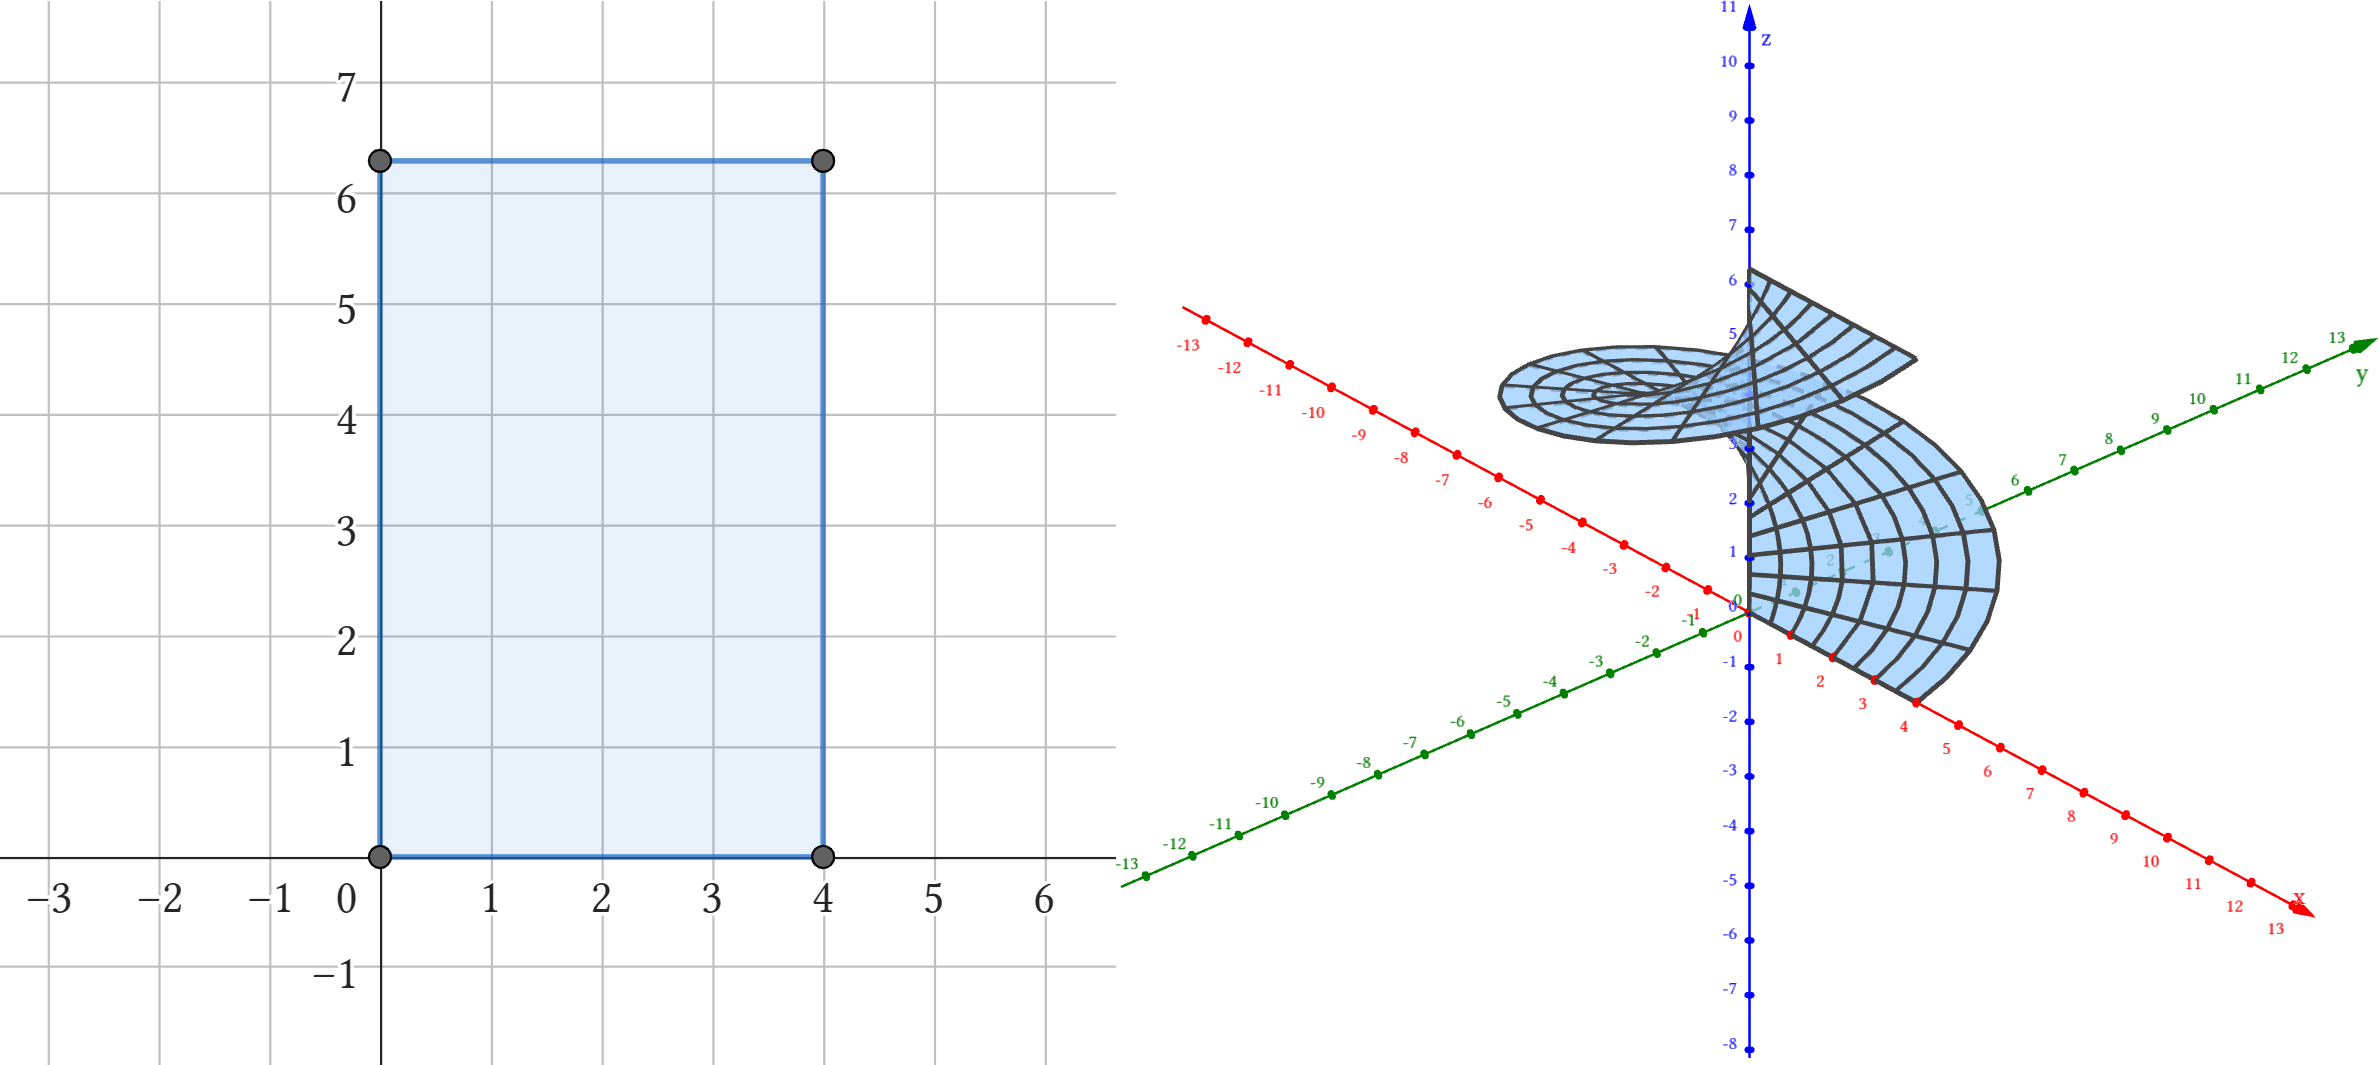
\includegraphics[width=0.75\textwidth]{images/II.4.4.png}
    \caption{由例\ref{exp:II.4.7}的参数方程定义的曲面。}
    \label{fig:II.4.4}
\end{figure}

\begin{definition}[函数的水平集]\label{def:II.4.4}
    函数$\mathbf{f}:\mathbb{R}^n\supset D\rightarrow\mathbb{R}^m$的\emph{水平集(level set)}是其定义域$D$的子集$S=\left\{\mathbf{r}|\mathbf{f}\left(\mathbf{r}\right)=\mathbf{a}\right\}$,其中$\mathbf{a}\in\mathrm{ran}\mathbf{f}$是某常向量\cite[\S7.1]{华工高数2009下}。
\end{definition}
\begin{example}\label{exp:II.4.8}
    设函数$f:\mathbb{R}^3\rightarrow\mathbb{R},f\left(\mathbf{r}\right)=r_1r_2+r_2r_3+r_3r_1$及其一个水平集$S=\left\{\mathbf{r}|f\left(\mathbf{r}\right)=1\right\}$。以$S$的元素$\left(r_1,r_2,r_3\right)$为坐标的点集构成的三维图形是怎样的?设$r_3=0$得到方程$r_1r_2=1$,这定义了$\mathbf{\hat{e}}_1$-$\mathbf{\hat{e}}_2$平面上的一条双曲线,这条双曲线是$S$的图像与$\mathbf{\hat{e}}_1-\mathbf{\hat{e}}_2$平面的截线。类似地,$S$与$\mathbf{\hat{e}}_2-\mathbf{\hat{e}}_3$、$\mathbf{\hat{e}}_1-\mathbf{\hat{e}}_3$平面的戴线也是类似的双曲线。更一般地,$S$是一个由一系列双曲线构成的曲面(如图\ref{fig:II.4.5}所示)。但是,按定义\ref{def:II.4.3},这不是函数$\mathbf{f}$的图像。
\end{example}
\begin{figure}[h]
    \centering
    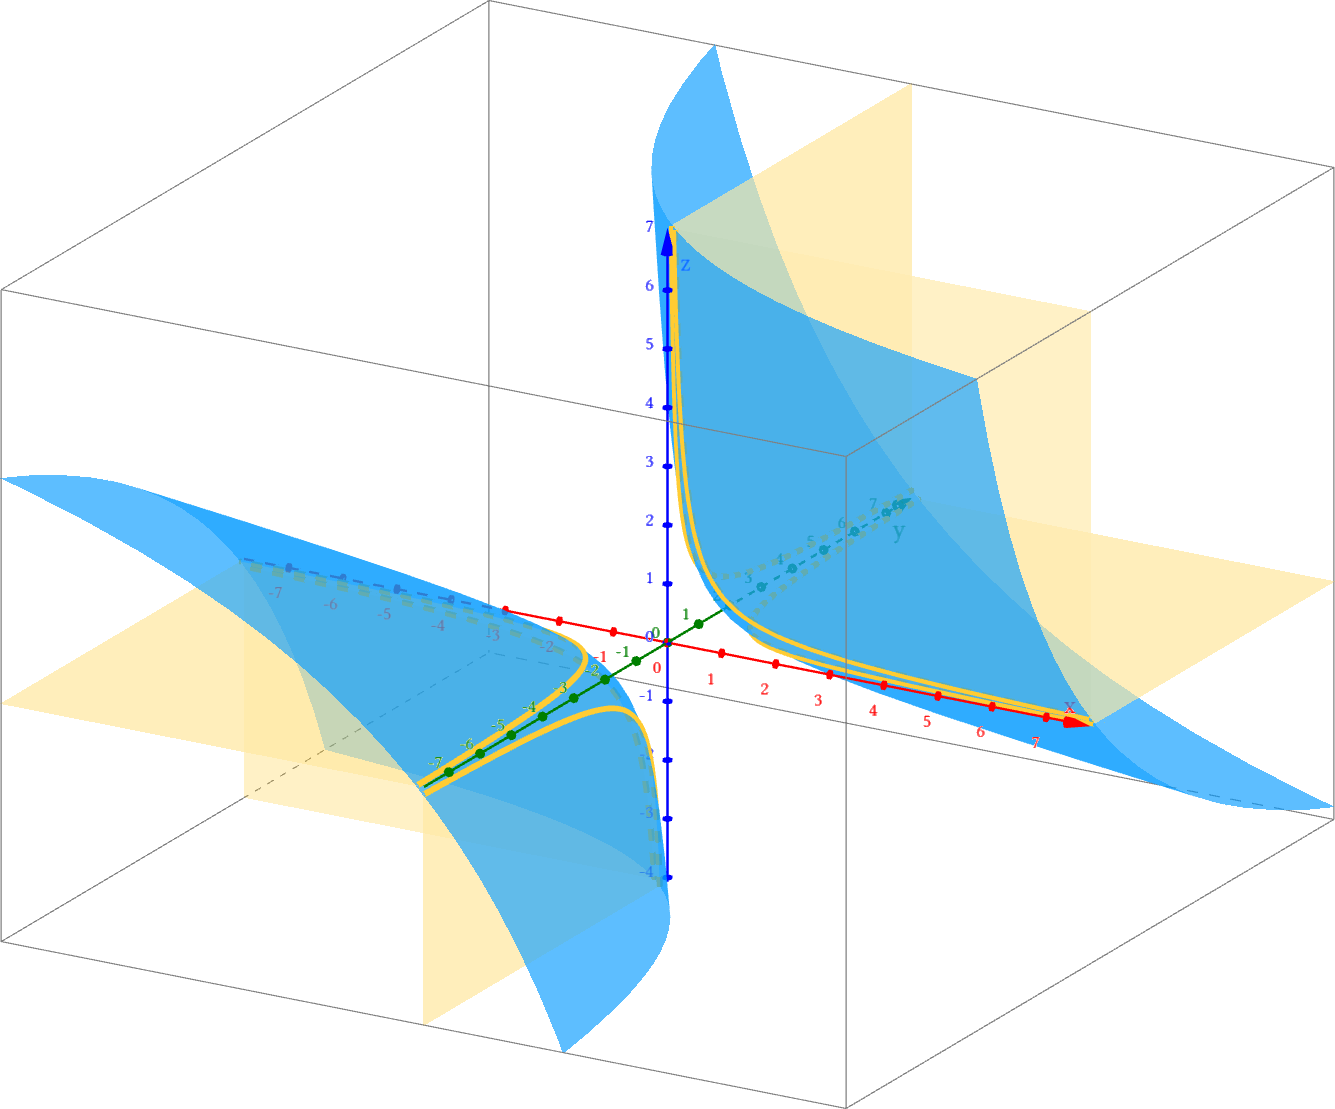
\includegraphics[width=0.75\textwidth]{images/II.4.5.png}
    \caption{函数$f\left(\mathbf{r}\right)=r_1r_2+r_2r_3+r_3r_1$的水平集$S=\left\{\left(x,y,z\right)|xy+yz+xz=1\right\}$。}
    \label{fig:II.4.5}
\end{figure}
总结以上例子,我们给一个函数画出来的图有以下三种情况:
\begin{enumerate}
    \item 如果$\mathbb{R}^{n+m}$的子集$S$是函数$\mathbf{f}:\mathbb{R}^n\rightarrow\mathbb{R}^m$的图像,则称$S$是由显函数定义的图像(例\ref{exp:II.4.4},\ref{exp:II.4.5},\ref{exp:II.4.6})。
    \item 如果$\mathbb{R}^{m}$的子集$S$是函数$\mathbf{f}:\mathbb{R}^n\rightarrow\mathbb{R}^m$的值域,则$S$是由参数方程定义的图像(例\ref{exp:II.4.7})。
    \item 如果$S$是函数$\mathbf{f}:\mathbb{R}^n\rightarrow\mathbb{R}^m$的一个水平集,则$S$是由隐函数定义的图像(例\ref{exp:II.4.8})。
\end{enumerate}

注意:只有第1种情况中$S$才是函数$\mathbf{f}$的图像,但我们经常通过第2、3种情况中的$S$来认识函数$\mathbf{f}$。
\end{document}